\documentclass[tikz,convert={outfile=\jobname.svg}]{standalone}
\usetikzlibrary{calc,patterns,snakes}
% \usetikzlibrary{...}% tikz package already loaded by 'tikz' option
\begin{document}
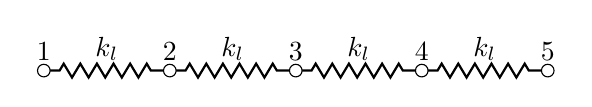
\begin{tikzpicture}[scale=0.4]
    \tikzstyle{spring}=[thick,decorate,decoration={zigzag,pre
        length=0.2cm,post length=0.2cm,segment length=6}]
    % Springs-Lines
    \draw[spring] (0,0) -- (4,0) node[above,pos=0.5] {$k_l$};
    \draw[spring] (4,0) -- (8,0) node[above,pos=0.5] {$k_l$};
    \draw[spring] (8,0) -- (12,0) node[above,pos=0.5] {$k_l$};
    \draw[spring] (12,0) -- (16,0) node[above,pos=0.5] {$k_l$};
    % Nodes
    \draw[fill = white] (0, 0) circle (.2) node[above] {$1$};
    \draw[fill = white] (4, 0) circle (.2) node[above] {$2$};
    \draw[fill = white] (8, 0) circle (.2) node[above] {$3$};
    \draw[fill = white] (12, 0) circle (.2) node[above] {$4$};
    \draw[fill = white] (16, 0) circle (.2) node[above] {$5$};
  \end{tikzpicture}
\end{document}